\documentclass[12pt]{article}
\usepackage{sbc-template}
\usepackage{url}
\usepackage{graphicx}
\usepackage{paralist}
\usepackage{epstopdf}
%\usepackage[pdftex]{graphicx}
\usepackage{longtable}
\usepackage[utf8]{inputenc}
\usepackage{scalefnt}
\usepackage{easylist}
\usepackage{multirow}
\usepackage{float}
\usepackage[section]{placeins}
\usepackage{paralist}
\usepackage[final]{pdfpages}
\usepackage[brazilian]{babel}
\usepackage{cite}
\def\UrlFont{\tt\scriptsize}

\sloppy

\title{Aferição de Qualidade de Código-Fonte em Gestão de Contrato Ágil com apoio de um ambiente de \textit{Data Warehousing}: um estudo de caso em uma autarquia da administração pública 
federal}
\author{Guilherme Baufaker Rêgo$^1$}
\address{Faculdade UnB Gama -- Universidade de Brasília
\email{gbre.111@gmail.com}
}

\begin{document}


\maketitle
% Seção do Resumo
\begin{resumo}

Atualmente, algumas organizações da Administração Pública Federal iniciam investimentos para adotar contratações de serviços de desenvolvimento de \textit{software} utilizando métodos ágeis. Nestes processos de contratação percebeu-se a lacuna sobre como aferir a qualidade interna do produto recebido. O objetivo deste trabalho foi propor uma solução automatizada, apoiada em um ambiente de \textit{data warehousing}, com intuito de aferir cenários de limpeza de código-fonte, que são indicadores de pedaços de código-fonte não coesos e com problemas de design. Visando a validação empírica da solução automatizada, realizou-se um estudo de caso no qual foi avaliado as 24 releases mensais do Sistema Integrado de Gestão e Conhecimento (SIGC) do IPHAN no qual foram identificados 397 cenários de limpeza de código-fonte em 914 classes, em um total de mais 300.000 linhas de código-fonte na 24ª release do SIGC. 

\end{resumo}

% Seção da Introdução
\section{Introdução}
\label{intro}

No desenvolvimento de software, há diversas variáveis, quer sejam de natureza ambiental ou técnica, que provavelmente impactarão desde a execução do processo de análise de requisitos até a implantação do software \cite{beckarticle1999}. Essa característica torna o processo de desenvolvimento pouco previsível e complexo, requerendo flexibilidade e personalização para ser capaz de responder às mudanças. 
Em consonância a esse movimento, órgãos da Administração Pública Federal (APF) também têm aderido a utilização de metodologias ágeis nos processos de desenvolvimento de software.

Recentemente, o Tribunal de Contas da União publicou o Acórdão no 2314/2013 \cite{TCU:2013}
que abordou a experiência do uso de práticas ágeis utilizadas na contratação realizadas por instituições públicas federais, como por exemplo, Banco Central do Brasil (BACEN), Instituto do Patrimônio Histórico e Artístico Nacional (IPHAN) Tribunal Superior do Trabalho (TST). 

A Instrução Normativa nº 4 \cite{IN04:2010}, que versa sobre o processo de Contratação de Soluções de Tecnologia da Informação pelos órgãos integrantes do Sistema de Administração dos Recursos de Informação e Informática do Poder Executivo Federal, enuncia um conjunto de boas práticas e um modelo de processo de contratações conforme visto na Figura \ref{processo}. 

\begin{figure}[h]
        \centering
        \label{processo}
            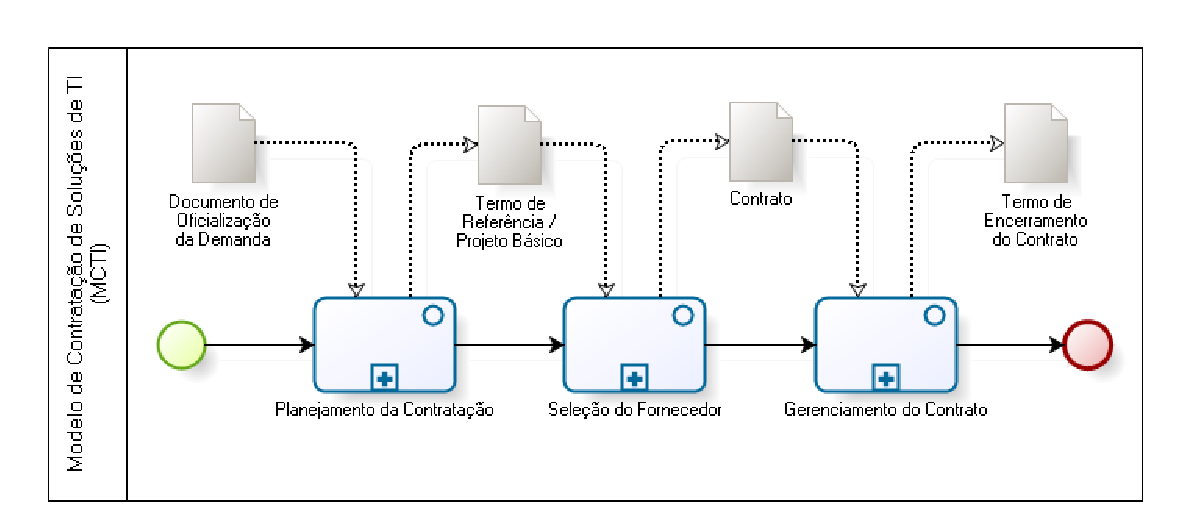
\includegraphics[scale=0.7]{figuras/MCTI.eps}
        \caption{Modelo de Processo de Contratações de Soluções de TI \cite{mcti}}
\end{figure}
\FloatBarrier

A fase de gerenciamento do contrato visa a acompanhar e garantir a adequada prestação do serviço e o fornecimento de bens que compõem a solução de TI, sendo que está disposto no art. 25, alínea b), que a avaliação da qualidade dos serviços realizados ou dos bens entregues e justificativas deve estar de acordo com os Critérios de Aceitação definidos em contrato, a cargo dos Fiscais Técnico e Requisitante do Contrato \cite{IN04:2010}.

Considerando: i) o princípio ágil de valoração de produto sobre documentação abrangente; ii) o foco na qualidade interna e iii) a necessidade das entidades da Administração Pública Federal do Poder Executivo aferirem a qualidade do produto entregue por seus fornecedores de desenvolvimento de software, conforme previsto na alínea b) do art. 25 da \cite{IN04:2010}, o objetivo desta pesquisa foi:


\begin{tabular}{p{3.5cm}p{8cm}}
Analisar & \textbf{o código-fonte} \\
com o propósito  de & \textbf{aferir a qualidade interna} \\
com respeito à & \textbf{aceitação do produto} \\
do ponto de vista do & \textbf{fiscal técnico do contrato} \\
no contexto da & \textbf{contratação de desenvolvimento de software por parte da Administração Pública Federal} \\
\end{tabular}
% Seção de Métricas e Cenários de Limpeza de Código-Fonte
\section{Processo de Medição da Qualidade Interna do Produto}

A qualidade interna do produto de software pode ser medida, ainda em ambiente de desenvolvimento, por meio da avaliação de estruturas internas que compõem o sistema de software \cite{ISO25023}, sendo que as métricas extraídas diretamente do código-fonte são bons indicadores de qualidade interna de produto \cite{beck2003test}, pois são métricas objetivas e com características como validade, simplicidade, objetividade, fácil obtenção e robustez \cite{Mills:1999}.  


Visando a identificação de um conjunto pequeno porém representativo de métricas de código-fonte que possam aferir a qualidade interna do produto de software em desenvolvimento, realizou-se uma revisão da literatura buscando identificar métricas para conceitos amplamente conhecidos como o tamanho do código-fonte que foi um dos primeiros conceitos mensuráveis do software; a complexidade que aumenta à medida que o software é evoluído, sendo que métricas de complexidade estão ligadas as métricas de tamanho \cite{Lehman1980b}; e métricas associadas a bom design no paradigma da orientação à objetos que permitiu evolução no desenvolvimento quando comparado ao paradigma procedural, fato que implicou a paradigma de orientação à objetos uma longa permanência na academia quanto na indústria de desenvolvimento de software \cite{Li1993}. Estas métricas foram reunidas e são apresentadas na Tabela \ref{orientacao}.     

	\begin{table}[!ht]
	\caption{Conjunto de Métricas de Código-Fonte}
	\addtolength{\belowcaptionskip}{6pt}
	\begin{center}
	\input{tabelas/orientacao-objeto.ltx}
	\label{orientacao}
	\end{center}
	\end{table}
	\FloatBarrier

Em um trabalho recente sobre a análise de métricas de código-fonte, foi observado o comportamento estatístico das métricas de código-fonte de 38 projetos de software livre com mais de 100.000 downloads em um esforço de análise de mais de 300.000 classes. Entre os softwares analisados estão Tomcat, OpenJDK, Eclipse, Google Chrome, VLC e entre outros que foram desenvolvidos em C, C++ e Java \cite{Meirelles2013}. Neste trabalho, concluiu-se que há valores muitos frequentes, frequentes, pouco frequentes e não frequentes para softwares escritos em uma mesma linguagem de programação. Ao considerarmos a linguagem Java e o softwares que obtiveram os melhores resultados, como Eclipse e o OpenJDK 8, obtiveram-se as configurações tal como se mostra na Tabela \ref{tab:good-metrics}.  


	\begin{table}[!ht]
	\caption{Configurações para os Intervalos das Métricas}
	\addtolength{\belowcaptionskip}{2pt}
	\begin{center}
	\input{tabelas/metricas.ltx}	
	\label{tab:good-metrics}
	\end{center}
	\end{table}
	\FloatBarrier

Em outros trabalhos como os de Marinescu  \cite{marinescu2005measurement}, Moha \cite{moha2010decor} e Rao \cite{rao2007detecting}, foi mostrado é possível detectar pedaços de código-fonte que podem ser melhorados, conhecidos como \textit{code-smell} \cite{fowler1999refactoring}, com a utilização de métricas de código-fonte como forma de detecção. Embasado em alguns destes trabalhos, \cite{Machini2010} construiu um mapeamento entre as métricas de código-fonte e as técnicas e práticas propostas por \cite{Martin2008} e \cite{beck2007implementation} de forma a construir cenários que indicam a possibilidade de melhoria no código-fonte.

Considerando alguns cenários do trabalho de Machini \cite{Machini2010} como base, foram construídos mapeamentos chamados de cenários de limpeza de código-fonte, que são mostrados Tabela \ref{tab:cenarios}. Cada cenário foi identificado por um nome, características da disposição do código-fonte, recomendações a fim de eliminar o pedaço de código não coesa e a forma de detecção pelos intervalos de frequência do trabalho de Meirelles \cite{Meirelles2013} que é compatível também com a forma de detecção apresentada nos trabalhos de Marinescu, Moha e Rao.
	
	\begin{table}[H]
	\centering
	\caption{Cenários de Limpeza de Código-Fonte}
	\addtolength{\belowcaptionskip}{6pt}
	\input{tabelas/cenarios.ltx}	
	\label{tab:cenarios}
	\end{table}
	\FloatBarrier

A partir da identificação dos cenários de limpeza de código-fonte e da contagem do número de classes em uma determinada \textit{release} do software, criou-se Taxa de Aproveitamento de Oportunidade de Melhoria de Código-Fonte como uma indicador objetivo de melhoria da qualidade do código-fonte, sendo que este é descrito conforme a Equação \ref{eqn01}.

\begin{equation}
\label{eqn01}
T_r =   \frac{{{Ce_r}}}{{Cl_r}}
\end{equation}

onde $ Ce_r $ é o total de cenários de limpeza em uma release e $ Cl_r $ é a quantidade classes na mesma release.

Com a identificação em um processo automatizado dos cenários e o cálculo da taxa de aproveitamento de oportnunidades, é possivel fornecer meios de verificação da qualidade código-fonte aos fiscais técnicos do contratos de desenvolvimento de software, de forma a introduzir a cultura de melhoria contínua da qualidade interna do produto em ciclos futuros de desenvolvimento do software. 



% Seção da Solução com o Uso de DW
\section{Solução para Automação do Processo de Medição da Qualidade Interna do Produto}
\label{sec:solucao}

Visando atingir a automação do processo de medição de qualidade interna do produto por meio de técnicas não intrusivas no ambiente de desenvolvimento de software, realizou-se uma revisão bibliográfica da literatura em busca de ambientes de informação permitissem o uso de ferramentas (não intrusivas) para automatizar a coleta e o uso de sofisticadas técnicas de análise de dados \cite{Gopal2005} . Trabalhos como o de Palza \cite{Palza2003},  Ruiz \cite{Ruiz2005}, Castellanos \cite{Castellanos2005},  Becker \cite{Becker2006}, Folleco \cite{Folleco2007} e Silveira \cite{Silveira2010}, evidenciaram que ambientes de \textit{Data Warehousing} são boas soluções para se automatizar um programa de métricas em processos de desenvolvimento de software.

\textit{Data Warehousing} é uma coleção de tecnologias de suporte à decisão disposta a capacitar os responsáveis por tomar decisões a fazê-las de forma mais rápida \cite{chaudhuri1997} \cite{andre2000}. Em outras palavras, trata-se de um processo para montar e gerenciar dados vindos de várias fontes, com o objetivo de prover uma visão analítica de parte ou do todo do negócio em repositório central chamado de \textit{data warehouse} \cite{gardner1998} \cite{Kimball2002}. A arquitetura de um ambiente de \textit{data warehousing} pode ser vista na Figura \ref{arquitetura}. 

\begin{figure}[ht!]
\centering
\includegraphics[keepaspectratio=false,scale=0.14]{figuras/Dwing.eps}
\caption{Arquitetura do Ambiente de \textit{Data Warehousing}}
\label{arquitetura}
\end{figure}
\FloatBarrier


Na Figura \ref{arquitetura}, as setas 1 e 2 representam o processo de \textit{Extraction-Transformation-Load (ETL)} que é o processo de extração, transformação e carga dos dados de forma automática e não intrusiva ao ambiente de desenvolvimento. Este processo pode consumir até 85\% de todo o esforço em um ambiente de \textit{Data Warehousing} \cite{Kimball2002}; A seta 3 representa as consultas \textit{On-Line Analytical Processing (OLAP)} que são operações de consulta e análise flexíveis realizadas sobre \textit{data warehouse}projetado sobre um modelo dimensional \cite{Kimball2002} \cite{Codd1993}; A seta 4 representa a visualização dos dados em forma de gráficos, tabelas ou painéis customizáveis conhecidos como \textit{dashboards}.


A implementação do ambiente de \textit{data warehousing} mostrado na figura \ref{arquitetura} se deu pela ferramenta Analizo\footnote{Disponível em \url{http:/http://analizo.org/}}, responsável por coletar as métricas de código-fonte, a suite Pentaho BI Community\footnote{Disponível em \url{http://community.pentaho.com/}}, que dispõe de ferramentas de ETL e OLAP, um banco de dados MariaDB\footnote{Disponível em \url{http://mariadb.org/}} modelado sobre um modelo dimensional e o plugin Saiku Analitics\footnote{Disponível em \url{http://meteorite.bi/saiku}} para visualização de dados. 
% Seção do Estudo de Caso
\section {Estudo de Caso}

Visando a validação da solução apresentada na Seção \ref{sec:solucao}, foram consultadas as instituições citadas pelo Acórdão no 2314/2013 \cite{TCU:2013}. Dentre elas, o Instituto do Patrimônio Histórico e Artístico Nacional (IPHAN) que é autarquia da administração pública federal responsável pela gestão de diversos processos de preservação do patrimônio cultural, permitiu o acesso ao processo, documentos e o código-fonte Sistema Integrado de Gestão do Conhecimento (SICG), um dos primeiros softwares desenvolvidos sob um contrato de terceirização de serviços com a utilização de metodologias ágeis.

O Sistema Integrado de Gestão do Conhecimento (SICG) teve como objetivo automatizar o processo de trabalho decorrente da metodologia de inventário, cadastro, normatização, fiscalização, planejamento e análise e gestão do patrimônio material. Esta solução de software foi construída na linguagem Java com a utilização de\textit{frameworks} como VRaptor e Hibernate, durante 24 \textit{releases} mensais. Possui um total 39.790 linhas de código distribuídas em 914 classes.

\subsection{Protocolo do Estudo de Caso}
Seguindo a metodologia proposta por Wohlin \cite{wohlin2012experimentation}, foi construído um protocolo de estudo de caso que foi baseado em Brereton \cite{brereton2008using} quanto aos aspectos gerais e Yin \cite{yin2011applications} com relação as ameaças à validade do estudo. 

O objeto do estudo de caso é o ambiente de DWing projetado e implementado conforme apresentado na seção 3. A fonte de coleta dos dados, foi o código fonte do SICG. A partir do objetivo da pesquisa, foram elaborados objetivos específicos do estudo de caso utilizando o GQM \cite{Basili96b}. Nesta abordagem cada objetivo específico derivou uma série de questões específicas que são respondidas com métricas específicas, tal como se mostra na Tabela \ref{tbl:obj}

\begin{table}[ht]
\centering
\input{tabelas/objetivos.ltx}
\caption{Objetivos Específicos do Estudo de Caso}
\label{tbl:obj} 
\end{table}
\FloatBarrier


Com relação as ameaças citadas por Yin, a validade de construção pôde ser obtida com utilização da abordagem GQM para selecionar indicadores que representem a realidade conhecida. Com relação a validade interna do estudo está garantida quando se consegue observar as relações causais e todos os elementos que as compõem. No presente estudo de caso, a taxa de aproveitamento de oportunidades de refatoração é diretamente dependente da quantidade de cenários de limpeza identificados desde que o número de classes permaneça o mesmo. Quanto a validade externa, destaca-se que a utilização de um estudo de caso não é suficiente para generalizar os resultados deles obtidos, sendo necessário a utilização de estudo em múltiplos casos, a fim de comprovar resultados genéricos \cite{yin2011applications}. Com relação a confiabilidade, a partir da documentação da implementação do ambiente de \textit{Data Warehousing} conjuntamente com o protocolo de estudo de caso e as bases de dados das métricas de código-fonte, garante-se a repetição do estudo de caso e por conseguinte a confiabilidade.

\subsection{Execução e Resultados do Estudo de Caso}
\label{sec:resultados}
Para analisar os cenários de limpeza de código-fonte, foram extraídas as métricas de código-fonte de cada classe e analisadas conforme a Tabela \ref{tab:cenarios}. Para cada \textit{release}, foram identificados, conforme a Figura \ref{fig:cenarios-release}, os cenários de limpeza de código-fonte. Para se mostrar maior nível de detalhes dos cenários de limpeza de código-fonte, realizou-se uma consulta OLAP de \textit{Drill-Down}, que tem objetivo de expor mais detalhes na visualização dos dados \cite{Kimball2002}, sobre o modelo dimensional do \textit{data warehouse}. 


\begin{figure}[ht!]
\centering
\includegraphics[keepaspectratio=true,scale=0.43]{figuras/total-cenario-tipo.eps}
\caption{Total de Cenários de Limpeza de Código-Fonte identificados por cenário e \textit{Release}}
\label{fig:cenarios-release}
\end{figure}
\FloatBarrier

A fim de se obter o número total de cenários de limpeza por cada uma das releases de software analisadas, como se observa na Figura \ref{fig:cenarios-total}, foi realizada uma consulta OLAP de \textit{Drill-Up}, que tem o objetivo de agregar o nível de visualização dos dados \cite{Kimball2002}, sobre os dados obtidos na Figura \ref{fig:cenarios-release}.

\begin{figure}[ht!]
\centering
\includegraphics[keepaspectratio=true,scale=0.45]{figuras/total-cenarios-release.eps}
\caption{Total de Cenários de Limpeza de Código-Fonte por Release}
\label{fig:cenarios-total}
\end{figure}
\FloatBarrier

Conforme é possível observar nas Figuras \ref{fig:cenarios-release} e \ref{fig:cenarios-total}, foram detectados mais cenários de limpeza de código-fonte dos tipos \textbf{Complexidade Estrutural}, que corresponde entre 55\% a 68\% da quantidade total de cenários identificados; \textbf{Classe Pouco Coesa} e \textbf{Interface dos Métodos} respectivamente. Os três Cenários de Limpeza com menor número de incidências foram \textbf{Classe com Muita Exposição}, \textbf{Classe com Muitos Filhos} e \textbf{Classe com Métodos Muito Grande e/ou com muitos condicionais}.

Considerando que é importante conhecer as classes com maior incidência de problemas com relação limpeza de código-fonte, foram identificadas, como se mostra na Figura \ref{fig:worst-10-cenarios}, as 10 classes que apresentaram a maior quantidade de cenários de limpeza de código-fonte. Para se obter a informação desta consulta foram necessária uma consulta OLAP de \textit{Drill Down} sobre algumas dimensões e outra de \textit{Slice and Dice}, que tem o objetivo de selecionar os dados, sobre o resultado a consulta de \textit{Drill-Down}.    

\begin{figure}[ht!]
\centering
\includegraphics[keepaspectratio=true,scale=0.55]{figuras/10-best.eps}
\caption{As 10 classes com maior número identificado de Cénarios de Limpeza}
\label{fig:worst-10-cenarios}
\end{figure}
\FloatBarrier

Com a quantidade de classes e o total de cenários de limpeza de código-fonte, foi possível calcular a Taxa de Aproveitamento de Oportunidade de Melhoria de Código-Fonte por cada release do software conforme se mostra na Figura \ref{fig:taxa-cenarios}.

\begin{figure}[H]
\centering
\includegraphics[keepaspectratio=true,scale=0.38]{figuras/taxa-parcial.eps}
\caption{Taxa de Aproveitamento de Oportunidades de Melhoria de Código-Fonte}
\label{fig:taxa-cenarios}
\end{figure}
\FloatBarrier

Observa-se, por meio da Figura \ref{fig:taxa-cenarios}, que o valor da Taxa de Aproveitamento de Oportunidade de Melhoria de Código-Fonte possui uma tendência entre 0,4 a 0,5. Este fato pode indicar duas hipóteses: a primeira de que o projeto cresceu em uma taxa muito maior que a quantidade de cenários de limpeza, indicando assim uma estabilidade na complexidade do projeto; ou que não foram promovidas atividades de melhoria de código-fonte ao longo das 24 releases.

% Seção de Conclusão e Trabalhos Futuros
\section{Conclusões e Trabalhos Futuros}


Com relação a execução do estudo de caso, foi possível mostrar que a automação do processo de medição da qualidade interna do produto de software (objetivo específico OE1)  é possível de ser realizada de maneira contínua e automatizada por meio do ambiente de \textit{data warehousing}, pois além da automação da coleta de um volume de dados de díficil verificação manual (39.000 linhas de código-fonte e 914 classes na 24ª release), foram automatizados desde a interpretação dos cenários de limpeza de código-fonte, o cálculo da taxa de aproveitamento das oportunidades de melhoria do código-fonte, até a exibição dos dados em tabelas e gráficos.

Com os resultados apresentados na Seção \ref{sec:resultados}, verifica-se que uma outra contribuição ambiente de \textit{data warehousing} foi alcançada por meio das consultas OLAP que permitiram flexibilidade necessária para se avaliar tanto em nível de projeto (objetivo específico OE2), quanto em nível local (objetivo específico OE3) a saúde do projeto com relação a qualidade do código-fonte. Por meio de um ambiente de \textit{data warehousing} semelhante ao apresentado, os fiscais técnicos dos contratos podem contar com mecanismos que venham automatizar a atividade de aferição da qualidade do código-fonte, de forma seja possível definir níveis de aceitação de produto.
Como esse estudo ocorreu na fase final do contrato, não foi possível analisar a eficiência e eficácia da medição do aproveitamento de oportunidades de melhoria de código-fonte. Entretanto, com a solução apresentada, foi possível medir o comportamento da taxa de aproveitamento de oportunidades de melhoria do código-fonte. Porém, a partir dela, não foi possível fazer conslusões mais objetivas de forma a auxiliar o fiscal técnico quanto a aceitação/rejeição do produto contratado, atendendo assim, parcialmente ao objetivo específico OE4.

Os resultados deste trabalho sugerem que o uso do ambiente proposto pode auxiliar a atividade de aferição da qualidade do produto por parte do fiscal técnico de contratos, além de auxiliá-lo a ter uma atitude propositiva ao apresentar os argumentos questionando a qualidade interna do software desenvolvido. Entretanto, trata-se de um estudo preliminar, que carece de maior aprofundamento e análises.

A partir da análise de uma amostragem de projetos, estatisticamente significativa, estudos futuros poderiam, por exemplo: identificar valores aceitáveis de nível de qualidade interna e identificar valores de referência para a taxa de oportunidade de melhoria de código-fonte.





\bibliographystyle{sbc}
\scalefont{.9}
\bibliography{myReferences}
\end{document}

